This chapter explore the method to further improve the performance levels of propsed load balancer.

Then performance levels in the 10Gbps environment is discussed.
Novel XDP load balancer is discussed.

\section{Load balancer for 10Gbps environment}

\begin{figure}[h]
  \centering
  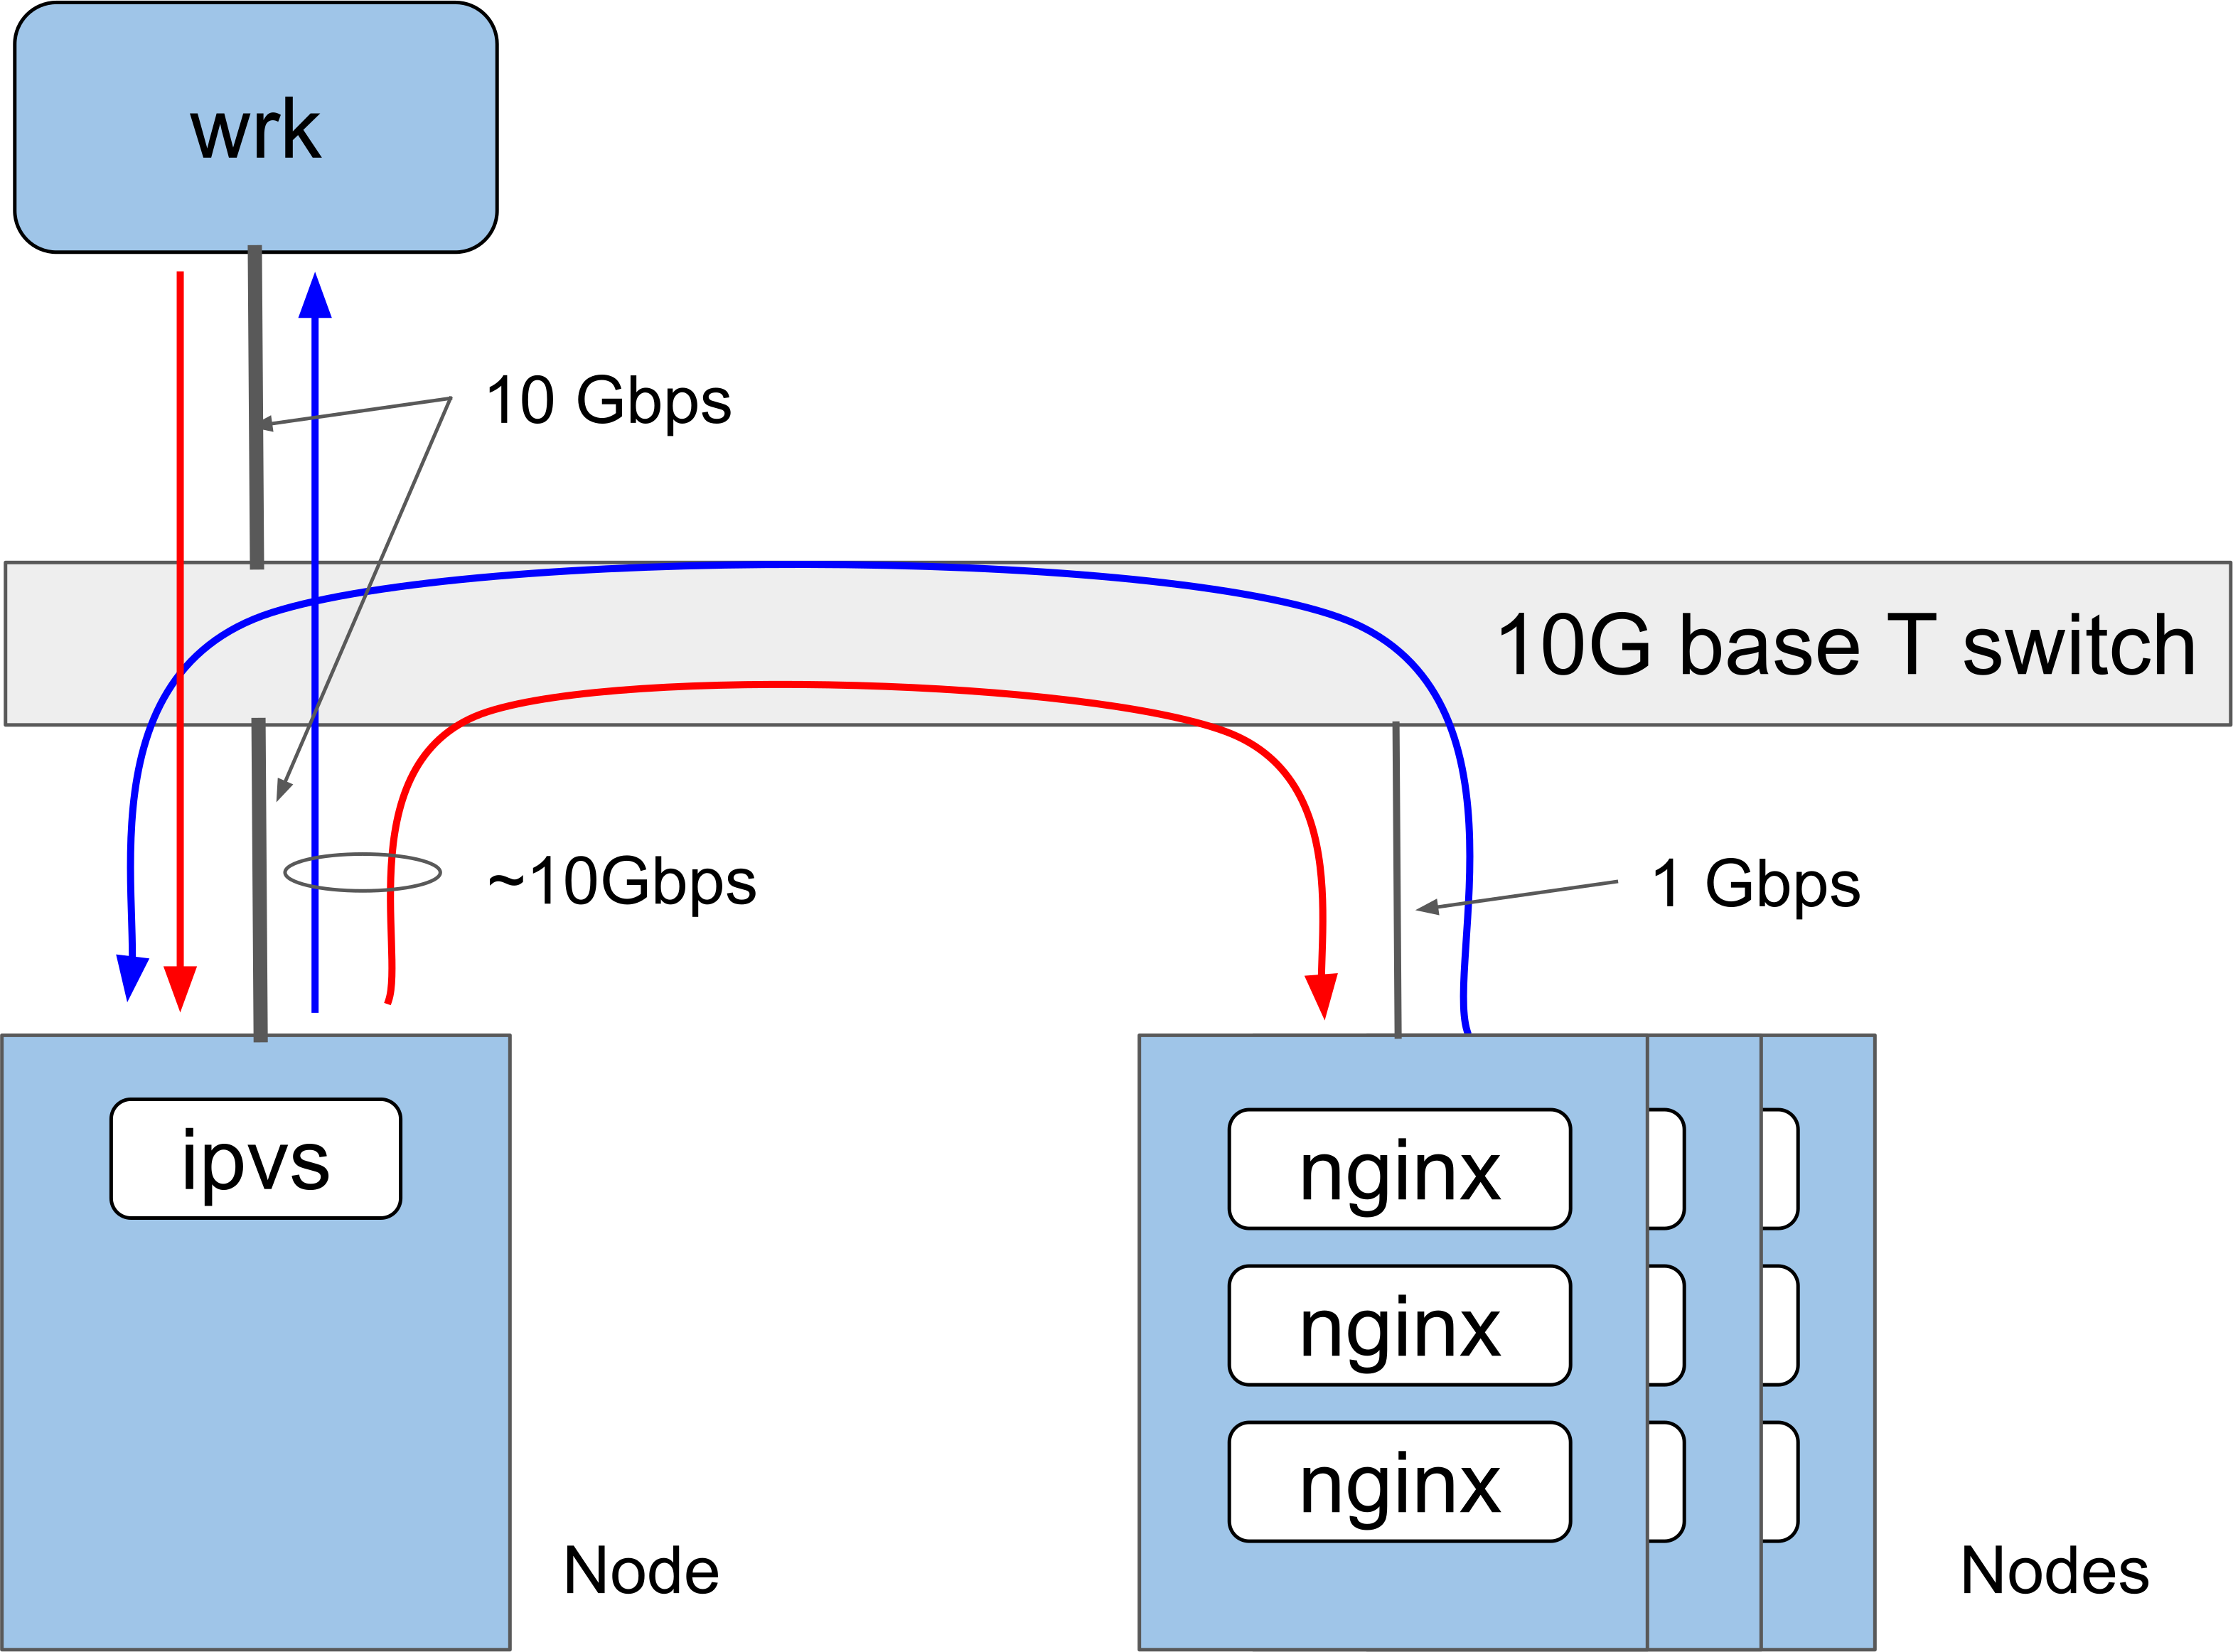
\includegraphics[width=0.8\columnwidth]{Figs/bench_10g}
  \caption{Physical configuration for 10Gbps measurement.}
  \label{fig:bench_10g}
\end{figure}

\begin{figure}[h]
  \centering
  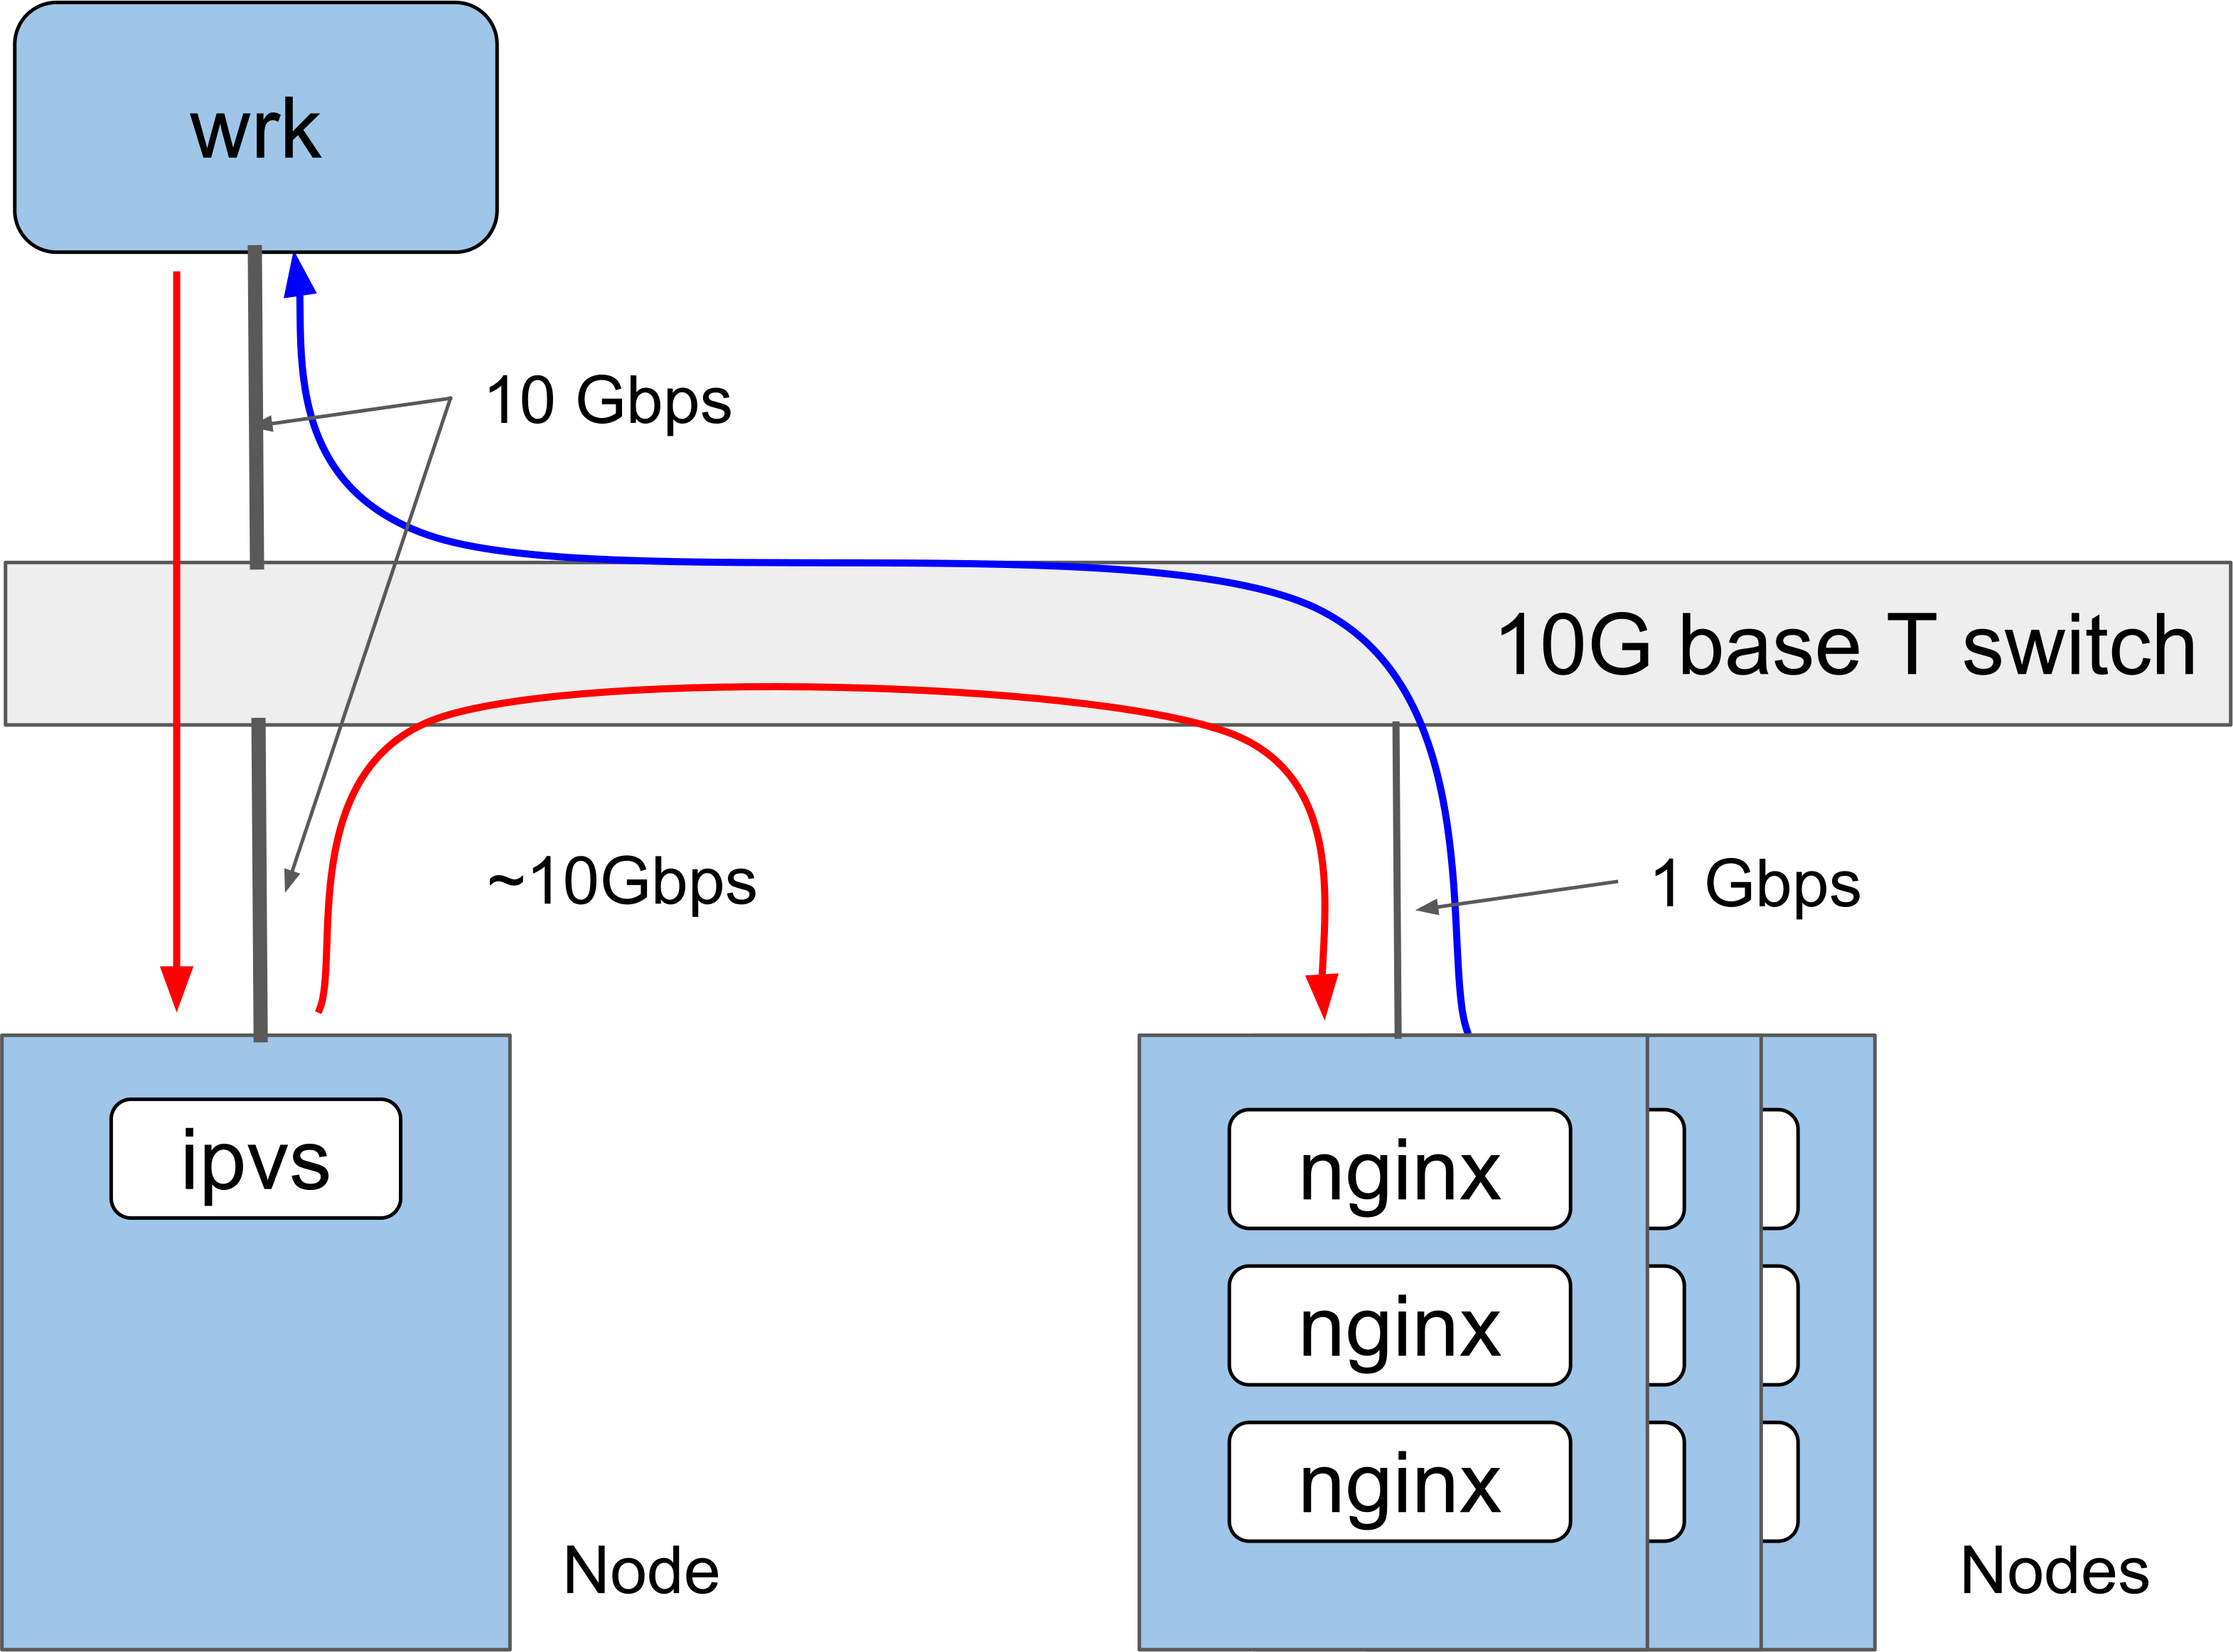
\includegraphics[width=0.8\columnwidth]{Figs/bench_10g_l3dsr}
  \caption{Physical configuration for L3DSR experiment.}
  \label{fig:bench_10g_l3dsr}
\end{figure}


\begin{figure}[t]
  \centering
  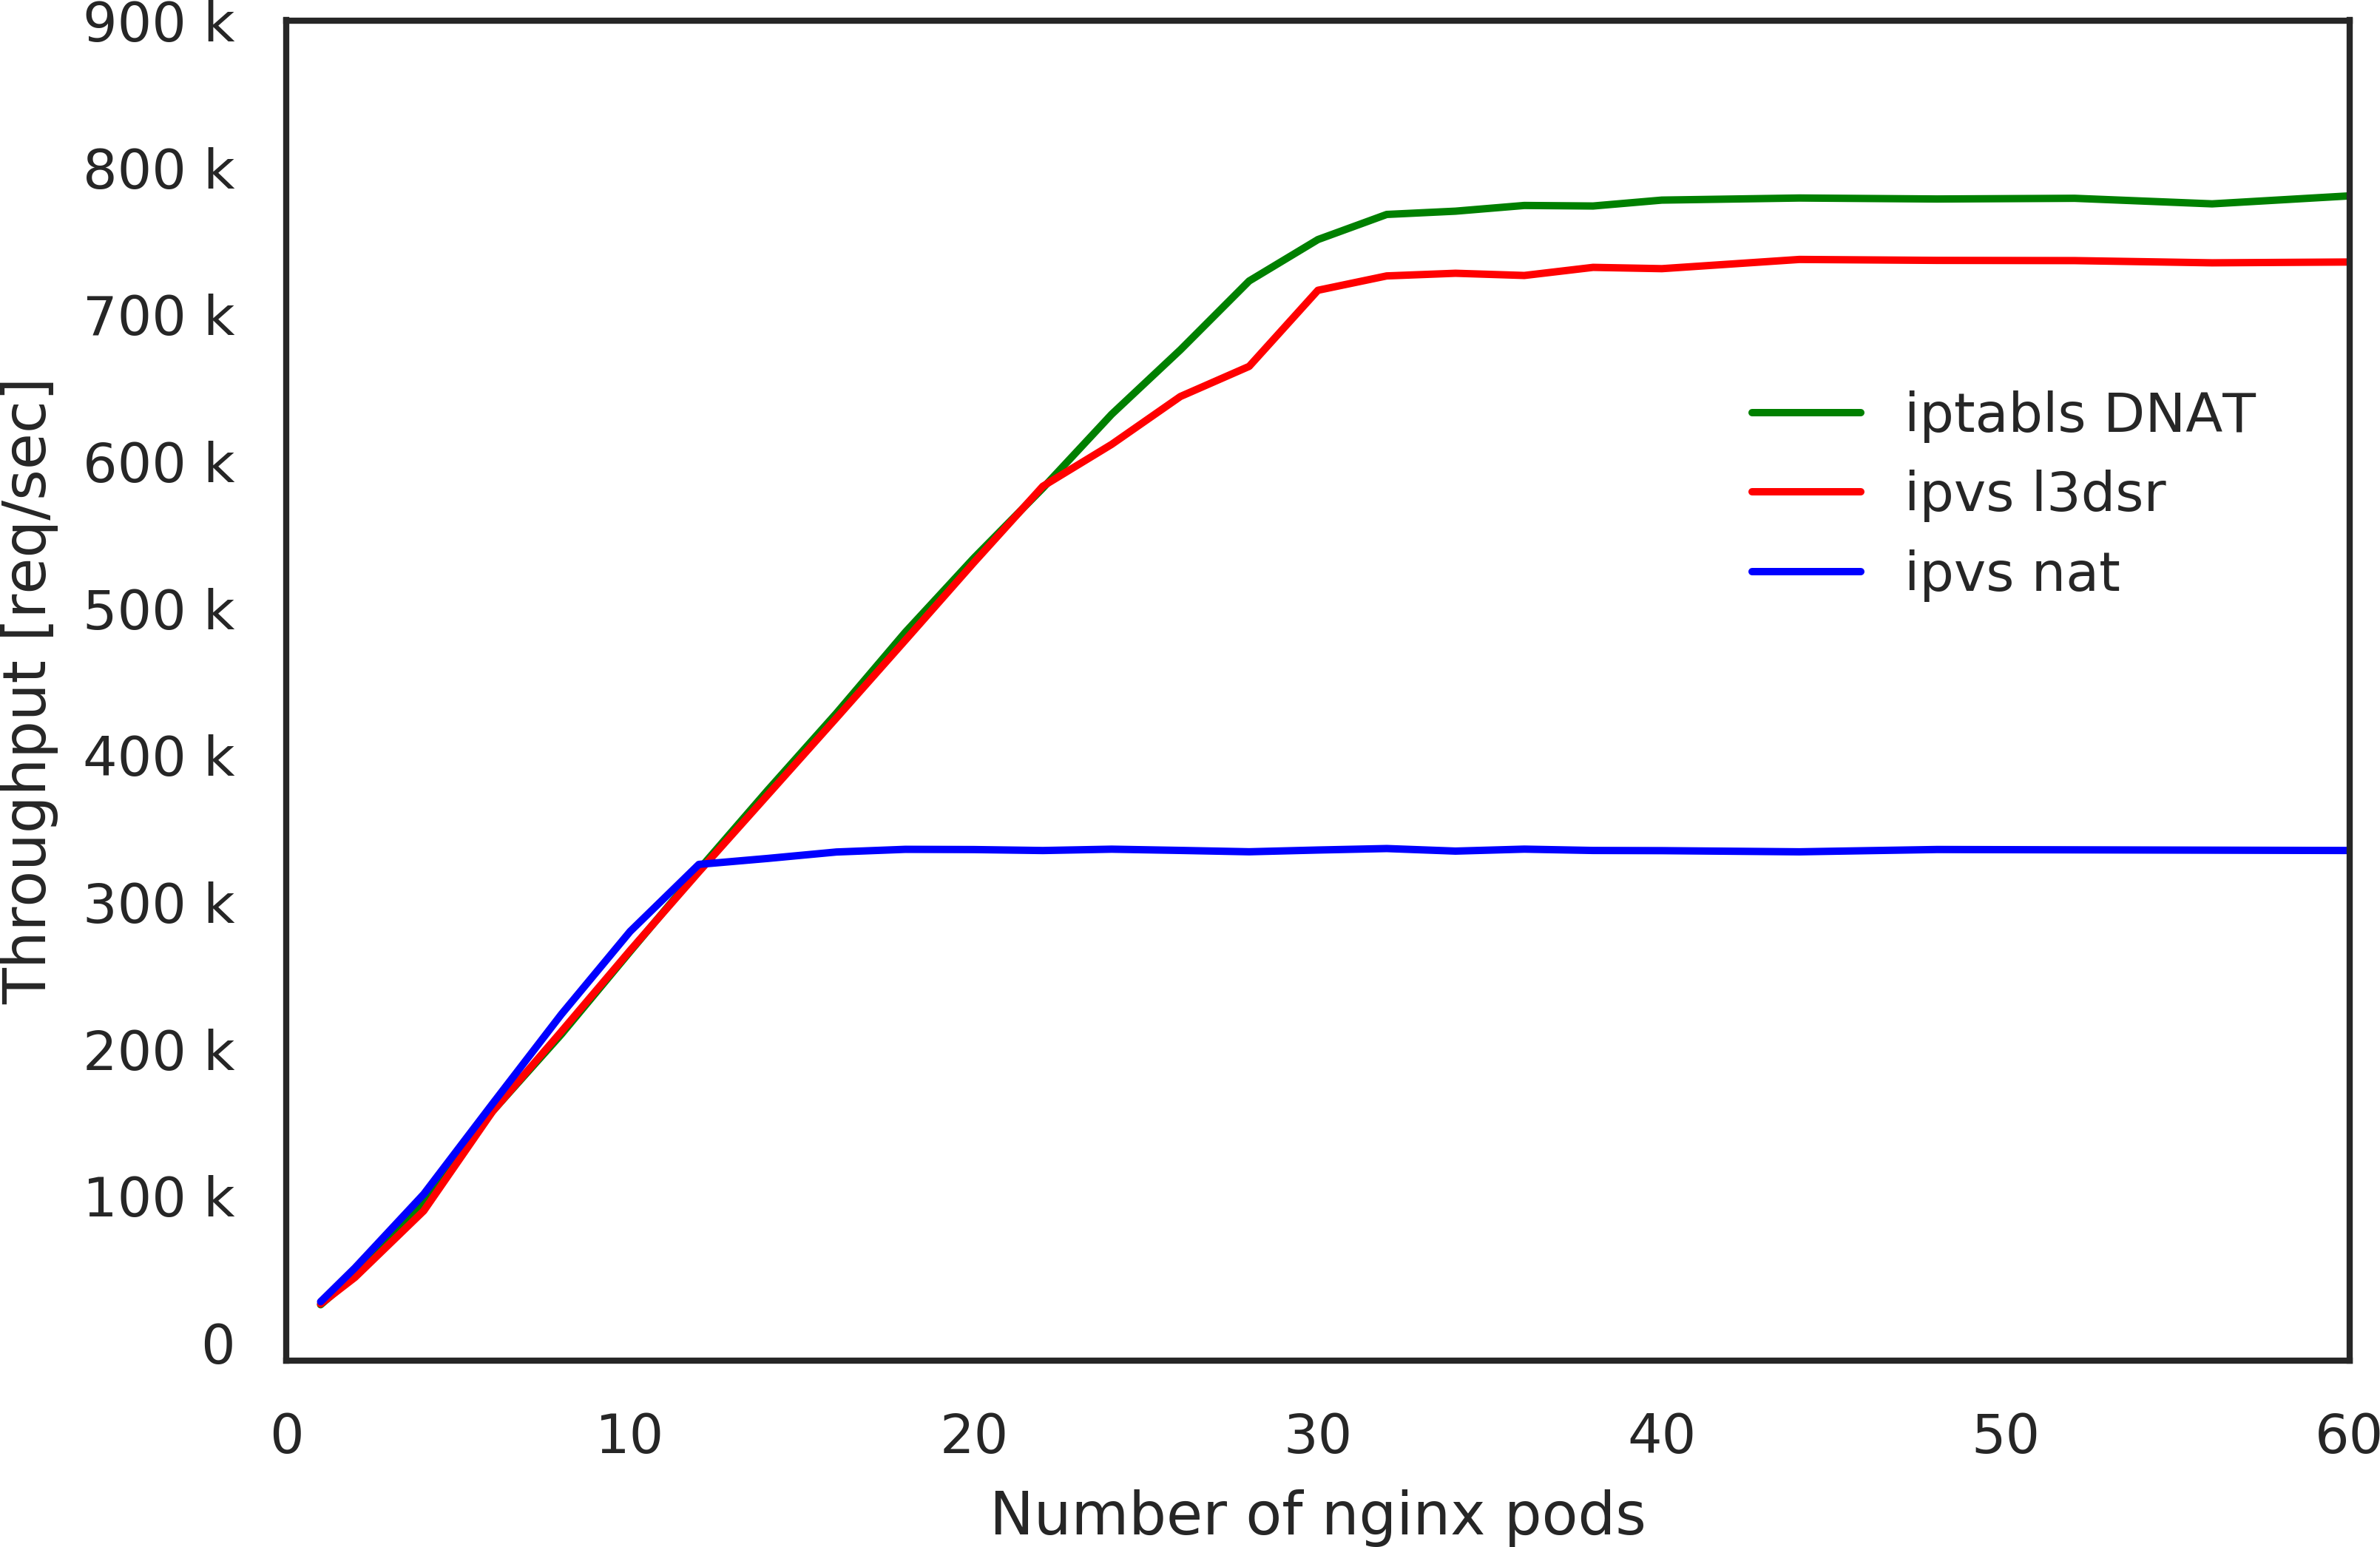
\includegraphics[width=0.8\columnwidth]{Figs/ipvs_l3dsr_10g.png}
  \caption{Throughput of ipvs l3dsr @10Gbps.}
  \label{fig:ipvs_l3dsr_10g.png}
\end{figure}

Figure~\ref{fig:ipvs_l3dsr_10g.png} shows the throughput of the ipvs-tun, ipvs masqurade mode togther with iptables DNAT.

\FloatBarrier

\section{XDP load balancer}

\section{Summary}



